\documentclass[conference]{IEEEtran}

\usepackage{cite}
\usepackage{amsmath,amssymb}
\usepackage{graphicx}
\usepackage{booktabs}
\usepackage{url}
\usepackage{tikz}
\usetikzlibrary{arrows.meta,positioning}

% A framed box that stands in for a photo until it is taken.
% Replace \placeholder{...} with \includegraphics[width=\columnwidth]{figures/<file>}.
\newcommand{\placeholder}[1]{%
  \fbox{\parbox[c][3.6cm][c]{0.92\columnwidth}{\centering\small\textbf{PHOTO PLACEHOLDER}\\[3pt]#1}}}

\newcommand{\vect}[1]{\boldsymbol{#1}}

\begin{document}

\title{Task-Space Typing with a Low-Cost Five-Joint Arm:\\Forward and Inverse Kinematics on the LeKiwi Robot}

% TODO: fill in the team members' names and NetIDs.
\author{\IEEEauthorblockN{NAME 1 (NetID), NAME 2 (NetID), NAME 3 (NetID)}
\IEEEauthorblockA{Team 20, ROB-GY 6003 Foundations of Robotics\\
New York University Tandon School of Engineering\\
Brooklyn, NY, USA}}

\maketitle

% =====================================================================
\begin{abstract}
Manipulation tasks are usually given as a position of the robot's tool, while the motors can only be commanded as joint angles. We developed forward kinematics (FK) and inverse kinematics (IK) for the five-joint arm of the LeKiwi mobile manipulator and used them to type words on a computer keyboard. FK is computed as a chain of axis--angle rotations about the joints' zero-pose axes. IK is solved with a damped-least-squares iteration on a finite-difference Jacobian that places the fingertip at a target point while keeping the finger vertical. Both run as Robot Operating System~2 (ROS~2) nodes that drive either a MuJoCo simulation or the real robot. In simulation, the FK matched the simulator's ground-truth fingertip with a median error of 0.02~mm over a 45~s trajectory spanning $30\times69\times30$~cm, and all keys registered for move times down to 0.25~s, with missed keys at 0.15~s and below. On the real robot, the arm typed the word ``pool'' with 4 of 4 letters correct and every press settled within 2.1--4.1~mm of its target. Lifting motions, however, stalled up to 44~mm short of the commanded height because the shoulder servo could not overcome gravity.
\end{abstract}

% =====================================================================
\section{Introduction}

A robot arm is driven in joint space, but tasks are usually given in task space, as a place the tool has to reach. In our case the tool is a finger and the place is a key. Forward kinematics maps the measured joint angles to the pose of the end effector, so the controller can compare where the tool is with where it should be. Inverse kinematics solves the opposite problem. It finds the joint angles that place the end effector at a desired pose, so that a task-space goal becomes a command the motors can execute. Any arm that is given goals as tool positions needs both~\cite{slides}.

This work applies FK and IK to the LeKiwi, a low-cost mobile manipulator built from hobby-grade serial-bus servos~\cite{lerobot}. Its arm has five revolute joints (shoulder pan, shoulder lift, elbow flex, wrist flex and wrist roll) and a parallel gripper. The end effector is defined as the tip of the gripper's fixed finger. The task is to press keys on a keyboard placed in front of the robot and spell a word. Software was developed and tested first against a MuJoCo model of the robot and a three-key simulated keyboard provided with the course material~\cite{for26}. The same ROS~2 nodes~\cite{ros2docs} were then run on the physical robot to type the word ``pool'' on a laptop keyboard.

The remainder of the paper is organized as follows. The Method section (Section~\ref{sec:method}) gives the mathematical details of the FK model, the damped-least-squares IK solver and the typing motion, and summarizes the control system in a block diagram. The Experiment Design section (Section~\ref{sec:experiment}) describes the simulated and physical setups and how the key positions and errors were measured. The Experimental Results section (Section~\ref{sec:results}) presents the FK validation, the positioning accuracy, the speed limit of typing and the real-robot typing run, and it discusses the problems we observed. The Conclusion (Section~\ref{sec:conclusion}) summarizes the strengths and weaknesses of the system.

% =====================================================================
\section{Method}
\label{sec:method}

\subsection{System overview}
Fig.~\ref{fig:block} shows the control system. All quantities are expressed in the robot's base frame, whose origin is at the centre of the base plate, with $x$ forward, $y$ to the left and $z$ up. The robot (simulated or real) publishes the measured joint angles $\boldsymbol{\theta}_m$. The FK node converts them into the estimated fingertip position $\hat{\vect{p}}$. A goal is given either as a letter to the keyboard typer or as a target position $\vect{p}^*$ to the end-effector control (EEControl) node, whose ROS node name is \texttt{inverse\_kinematics}. Both call the same IK solver, seeded with $\boldsymbol{\theta}_m$, and publish joint commands $\boldsymbol{\theta}_{c}$. The control is open loop in task space: the joint servos close the loop on angle, and the task-space error is not fed back.

\begin{figure}[t]
\centering
\resizebox{\columnwidth}{!}{%
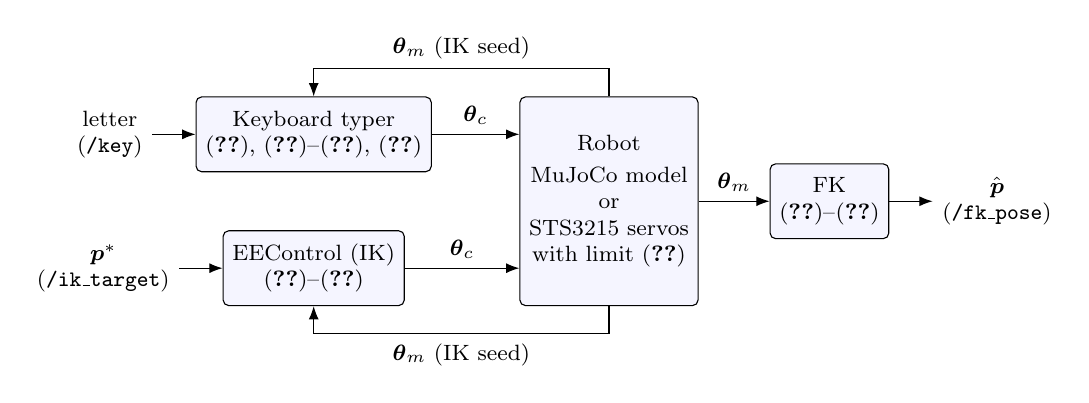
\begin{tikzpicture}[>=Latex, font=\footnotesize,
  box/.style={draw, rounded corners=2pt, align=center, minimum height=0.95cm, minimum width=2.3cm, fill=blue!4}]
  \node[box] (typer) at (0, 0.85) {Keyboard typer\\ \eqref{eq:waypoints}, \eqref{eq:task}--\eqref{eq:accept}, \eqref{eq:interp}};
  \node[box] (ik)    at (0,-0.85) {EEControl (IK)\\ \eqref{eq:task}--\eqref{eq:accept}};
  \node[left=0.55cm of typer, align=center] (key) {letter\\(\texttt{/key})};
  \node[left=0.55cm of ik, align=center] (tgt) {$\vect{p}^*$\\(\texttt{/ik\_target})};
  \node[box, minimum height=2.65cm, minimum width=2.1cm] (robot) at (3.75,0) {Robot\\[2pt] MuJoCo model\\ or\\ STS3215 servos\\ with limit \eqref{eq:clamp}};
  \node[box, minimum width=1.5cm] (fk) at (6.55,0) {FK\\ \eqref{eq:rodrigues}--\eqref{eq:fk}};
  \node[right=0.55cm of fk, align=center] (out) {$\hat{\vect{p}}$\\(\texttt{/fk\_pose})};
  \draw[->] (key) -- (typer);
  \draw[->] (tgt) -- (ik);
  \draw[->] (typer.east) -- node[above]{$\boldsymbol{\theta}_c$} (typer.east -| robot.west);
  \draw[->] (ik.east) -- node[above]{$\boldsymbol{\theta}_c$} (ik.east -| robot.west);
  \draw[->] (robot) -- node[above]{$\boldsymbol{\theta}_m$} (fk);
  \draw[->] (fk) -- (out);
  \draw[->] (robot.north) -- ++(0,0.35) -| node[pos=0.25, above]{$\boldsymbol{\theta}_m$ (IK seed)} (typer.north);
  \draw[->] (robot.south) -- ++(0,-0.35) -| node[pos=0.25, below]{$\boldsymbol{\theta}_m$ (IK seed)} (ik.south);
\end{tikzpicture}}
\caption{Block diagram of the control system. Numbers in parentheses refer to the equations in Section~\ref{sec:method}. Joint commands $\boldsymbol{\theta}_c$ travel on \texttt{/arm\_commands} and measured angles $\boldsymbol{\theta}_m$ on \texttt{/arm\_state}. The keyboard typer was used in simulation and the EEControl node on the real robot.}
\label{fig:block}
\end{figure}

\subsection{Forward kinematics}
The arm is described at its zero pose, where all joint angles are zero. For joint $k\in\{1,\dots,5\}$, $\vect{q}_k\in\mathbb{R}^3$ is a point on its rotation axis and $\vect{\omega}_k\in\mathbb{R}^3$ is the unit axis direction, with positive angles following the right-hand rule. The fingertip position and the finger's unit pointing direction at the zero pose are $\vect{p}_h$ and $\vect{d}_h$. Table~\ref{tab:params} lists these values, which were read from the MuJoCo model~\cite{for26}. The joint angles are $\boldsymbol{\theta}=[\theta_1,\dots,\theta_5]^T$.

The rotation of a vector $\vect{v}$ by an angle $\theta$ about a unit axis $\vect{\omega}$ is given by Rodrigues' formula~\cite{slides}:
\begin{equation}
\begin{aligned}
\vect{R}(\vect{\omega},\theta)\,\vect{v} = {}& \vect{v}\cos\theta + (\vect{\omega}\times\vect{v})\sin\theta\\
&+ \vect{\omega}\,(\vect{\omega}^T\vect{v})(1-\cos\theta).
\end{aligned}
\label{eq:rodrigues}
\end{equation}
The joint rotations are applied from the last joint to the first, starting from the zero pose,
\begin{equation}
\vect{p}^{(5)} = \vect{p}_h, \qquad \vect{d}^{(5)} = \vect{d}_h,
\label{eq:fkinit}
\end{equation}
\begin{equation}
\begin{aligned}
\vect{p}^{(k-1)} &= \vect{q}_k + \vect{R}(\vect{\omega}_k,\theta_k)\,(\vect{p}^{(k)}-\vect{q}_k),\\
\vect{d}^{(k-1)} &= \vect{R}(\vect{\omega}_k,\theta_k)\,\vect{d}^{(k)}, \qquad k=5,4,\dots,1,
\end{aligned}
\label{eq:fkstep}
\end{equation}
\begin{equation}
\vect{p}(\boldsymbol{\theta}) = \vect{p}^{(0)}, \qquad \vect{d}(\boldsymbol{\theta}) = \vect{d}^{(0)}.
\label{eq:fk}
\end{equation}
The joints are applied in reverse order because, while joint $k$ is being applied, joints $1,\dots,k-1$ are still at zero, so the axis of joint $k$ is still where the zero-pose table places it. The result is equivalent to the product-of-exponentials formula, with each exponential written out as~\eqref{eq:rodrigues}.

\begin{table}[t]
\centering
\caption{Zero-pose kinematic parameters of the arm (base frame)}
\label{tab:params}
\resizebox{\columnwidth}{!}{%
\begin{tabular}{@{}llll@{}}
\toprule
$k$ & Joint & $\vect{q}_k$ (m) & $\vect{\omega}_k$ \\
\midrule
1 & shoulder pan  & $(0.067, 0.000, 0.084)$ & $(0, 0, -1)$ \\
2 & shoulder lift & $(0.098, -0.018, 0.137)$ & $(0, 1, 0)$ \\
3 & elbow flex    & $(0.116, -0.017, 0.251)$ & $(0, 1, 0)$ \\
4 & wrist flex    & $(0.249, -0.015, 0.280)$ & $(0, 1, 0)$ \\
5 & wrist roll    & $(0.308, 0.005, 0.296)$ & $(-0.966, 0, -0.259)$ \\
\midrule
\multicolumn{4}{@{}l}{$\vect{p}_h = (0.413, 0.005, 0.310)$~m, \quad $\vect{d}_h = (0.966, 0, 0.259)$} \\
\bottomrule
\end{tabular}}
\end{table}

\subsection{Inverse kinematics}
Pressing a key requires the fingertip at a target point $\vect{p}^*$ with the finger pointing straight down, $\vect{d}^*=[0,0,-1]^T$. Both goals are stacked into a task vector, with the direction scaled by a weight $\lambda$ so that position dominates:
\begin{equation}
\vect{x}(\boldsymbol{\theta}) = \begin{bmatrix}\vect{p}(\boldsymbol{\theta})\\ \lambda\,\vect{d}(\boldsymbol{\theta})\end{bmatrix}\in\mathbb{R}^6,
\label{eq:task}
\end{equation}
\begin{equation}
\vect{e} = \begin{bmatrix}\vect{p}^*\\ \lambda\,\vect{d}^*\end{bmatrix} - \vect{x}(\boldsymbol{\theta}).
\label{eq:error}
\end{equation}
Only joints 1--4 are solved for. The wrist roll $\theta_5$ keeps its current value, because rolling about a vertical finger does not move the fingertip. Column $j$ of the $6\times4$ Jacobian $\vect{J}$ is estimated by finite differences, where $\delta$ is a small angle increment and $\vect{u}_j$ is the $j$-th unit vector:
\begin{equation}
\vect{J}_{j} = \frac{\vect{x}(\boldsymbol{\theta}+\delta\,\vect{u}_j)-\vect{x}(\boldsymbol{\theta})}{\delta}, \qquad j=1,\dots,4.
\label{eq:jacobian}
\end{equation}
The joint update follows damped least squares~\cite{slides}, with damping factor $\mu$ and the $6\times6$ identity $\vect{I}_6$:
\begin{equation}
\Delta\boldsymbol{\theta} = \vect{J}^T\left(\vect{J}\vect{J}^T+\mu^2\vect{I}_6\right)^{-1}\vect{e}.
\label{eq:dls}
\end{equation}
The damping keeps the step bounded near singularities, for example with the arm fully stretched. Each step is limited to $\Delta_{\max}$ per joint, and the result is saturated to the joint limits $[\theta_j^{\min},\theta_j^{\max}]$. With the saturation function $\sigma_a^b(z)=\min(b,\max(a,z))$,
\begin{equation}
\theta_j \leftarrow \sigma_{\theta_j^{\min}}^{\theta_j^{\max}}\!\left(\theta_j+\sigma_{-\Delta_{\max}}^{\Delta_{\max}}(\Delta\theta_j)\right), \qquad j=1,\dots,4.
\label{eq:clip}
\end{equation}
Equations~\eqref{eq:error}--\eqref{eq:clip} are iterated until $\|\vect{e}\|<10^{-6}$ or for at most 200 iterations. The iteration starts from the measured angles $\boldsymbol{\theta}_m$, so that the solution stays close to the current configuration. A solution is accepted only if the remaining position error is below a tolerance $\varepsilon$:
\begin{equation}
\left\|\vect{p}^*-\vect{p}(\boldsymbol{\theta})\right\| < \varepsilon.
\label{eq:accept}
\end{equation}
Otherwise the target is reported as unreachable and the arm does not move.

\subsection{Typing motion}
A key whose top is at $\vect{p}_k$ is pressed with three fingertip waypoints: a hover point at height $h$ above the key, a press point at depth $\delta_p$ below the key top, and the hover point again. With $\vect{e}_z=[0,0,1]^T$,
\begin{equation}
\vect{p}_{hov} = \vect{p}_k + h\,\vect{e}_z, \qquad \vect{p}_{prs} = \vect{p}_k - \delta_p\,\vect{e}_z.
\label{eq:waypoints}
\end{equation}
Aiming below the key top makes the press succeed despite millimetre-level errors. Each waypoint is converted to joint angles $\boldsymbol{\theta}_g$ with~\eqref{eq:task}--\eqref{eq:accept}, each IK solve seeded with the previous solution. Between a start configuration $\boldsymbol{\theta}_s$ and a goal $\boldsymbol{\theta}_g$, commands are interpolated linearly in joint space at rate $f$, over a move time $T$:
\begin{equation}
\boldsymbol{\theta}_c[n] = \boldsymbol{\theta}_s + (\boldsymbol{\theta}_g-\boldsymbol{\theta}_s)\min\!\left(1,\frac{n}{N}\right), \qquad N=\lfloor Tf\rfloor.
\label{eq:interp}
\end{equation}

\subsection{Real-robot servo interface}
On the real robot, the LeRobot driver~\cite{lerobot} limits how far a command may lead the measured angle in each 10~Hz control step. This prevents violent motions:
\begin{equation}
\theta_{c,j} \leftarrow \theta_{m,j} + \sigma_{-\Delta_s}^{\Delta_s}\!\left(\theta_{c,j}-\theta_{m,j}\right),
\label{eq:clamp}
\end{equation}
where $\Delta_s$ is the step limit. Each servo then runs its internal position controller toward $\theta_{c,j}$. Because the servo's effort grows with $\theta_{c,j}-\theta_{m,j}$,~\eqref{eq:clamp} also caps the effort available to fight gravity. Section~\ref{sec:results} returns to this. Table~\ref{tab:control} lists all controller parameters.

\begin{table}[t]
\centering
\caption{Controller parameters}
\label{tab:control}
\begin{tabular}{@{}lll@{}}
\toprule
Symbol & Meaning & Value \\
\midrule
$\lambda$ & direction weight in~\eqref{eq:task} & 0.05 \\
$\delta$ & finite-difference increment in~\eqref{eq:jacobian} & 0.01$^\circ$ \\
$\mu$ & damping in~\eqref{eq:dls} & 0.01 \\
$\Delta_{\max}$ & IK step limit in~\eqref{eq:clip} & 10$^\circ$ \\
$\varepsilon$ & acceptance tolerance in~\eqref{eq:accept} & 5~mm \\
$h$ & hover height in~\eqref{eq:waypoints} & 40~mm \\
$\delta_p$ & press depth in~\eqref{eq:waypoints} & 8~mm \\
$f$ & interpolation rate in~\eqref{eq:interp} & 20~Hz \\
$T$ & move time in~\eqref{eq:interp} & 1.5~s (default) \\
$\Delta_s$ & servo step limit in~\eqref{eq:clamp}, at 10~Hz & 5$^\circ$ \\
\bottomrule
\end{tabular}
\end{table}

% =====================================================================
\section{Experiment Design}
\label{sec:experiment}

\subsection{Simulated setup}
The simulation uses a MuJoCo model of the LeKiwi with a keyboard plate in front of the robot (Fig.~\ref{fig:simscene})~\cite{for26}. The plate holds three spring-loaded keys labelled \texttt{a}, \texttt{s} and \texttt{d}, with tops at $(0.300, \pm0.070\text{ or }0, -0.012)$~m. A key is 24~mm wide, travels 6~mm and counts as pressed at 3~mm. The simulator publishes the true fingertip position $\vect{p}_{true}$ on \texttt{/true\_fingertip} and an event on \texttt{/key\_pressed} for every press. This ground truth is available only in simulation, and it is what makes the following three error measures possible. With $\vect{p}_{tgt}$ the commanded press point and $\vect{p}_{FK}=\hat{\vect{p}}$ the FK estimate,
\begin{equation}
e_{pos} = \left\|\vect{p}_{true}-\vect{p}_{tgt}\right\|,
\label{eq:epos}
\end{equation}
\begin{equation}
e_{mod} = \left\|\vect{p}_{true}-\vect{p}_{FK}\right\|,
\label{eq:emod}
\end{equation}
\begin{equation}
e_{trk} = \left\|\vect{p}_{FK}-\vect{p}_{tgt}\right\|.
\label{eq:etrk}
\end{equation}
The position error $e_{pos}$ is the total error the task sees. The model error $e_{mod}$ measures the quality of the FK model, and the tracking error $e_{trk}$ measures how well the servos followed the IK command.

All topics were logged to CSV files by a recording node. Three simulated experiments were run:
\begin{enumerate}
\item \emph{FK validation}: a 45~s joint trajectory moving all five joints over wide ranges (shoulder pan $-80^\circ$ to $73^\circ$, wrist roll $-73^\circ$ to $71^\circ$), comparing $\hat{\vect{p}}$ with $\vect{p}_{true}$.
\item \emph{Typing accuracy}: typing \texttt{a}, \texttt{s} and \texttt{d} at $T=1.5$~s, evaluating~\eqref{eq:epos}--\eqref{eq:etrk} at the deepest point of each press, within 1.5~s of the press event.
\item \emph{Speed versus success}: typing the three keys at $T\in\{1.5, 1.0, 0.6, 0.4, 0.25, 0.15, 0.1\}$~s and counting registered presses.
\end{enumerate}

\begin{figure}[t]
\centering
\placeholder{MuJoCo screenshot: LeKiwi in front of the simulated keyboard (red \texttt{a}, green \texttt{s}, blue \texttt{d}), with the pink FK ball on the fingertip.}
\caption{Simulated setup: the LeKiwi model and the three-key keyboard. The FK estimate is drawn as a ball at the fingertip.}
\label{fig:simscene}
\end{figure}

\subsection{Physical setup}
On the real robot, a driver node replaces the simulator and publishes and subscribes to the same \texttt{/arm\_state} and \texttt{/arm\_commands} topics~\cite{lerobot,for26}. The FK and EEControl nodes ran unchanged on the robot's on-board computer. A laptop running a text editor was placed in front of the robot (Fig.~\ref{fig:setup}). The robot was turned so that the keys \texttt{P}, \texttt{O} and \texttt{L} lay about 0.28~m in front of and 0.12~m to the left of the base origin, inside the region the finger can reach while pointing down. The laptop's key repeat was disabled, so that a long press produces a single character.

The simulated arm has the geometry of an older arm version (SO-100), which differs from the real SO-101 by a few centimetres near the gripper~\cite{for26}. Measuring the keys with a ruler would therefore build this model error into the targets. Instead, the key positions were measured \emph{with the robot itself}. With the motors disabled, the finger was guided by hand onto each key, held down and pointing straight down (Fig.~\ref{fig:closeup}), and 0.5~s of $\hat{\vect{p}}$ was averaged. A target defined this way and later reached through the same FK model is consistent, so the model error cancels to first order. The home position was set 50~mm above the centroid of the three keys.

The word ``pool'' was typed by a script that sends the targets \texttt{home}, \texttt{p}, \texttt{home}, \texttt{o}, \texttt{home}, \texttt{o}, \texttt{home}, \texttt{l}, \texttt{home} on \texttt{/ik\_target}. It waits 0.7~s after each press command and 2.5~s after each home command. Success was judged from the characters appearing in the editor. Because no ground truth exists on the real robot, accuracy was measured with $\hat{\vect{p}}$, as the distance at which the fingertip settled from each target, just before the next command.

\begin{figure}[t]
\centering
\placeholder{Photo: the real LeKiwi facing the laptop keyboard, with the base frame axes ($x$ forward, $y$ left) drawn on.}
\caption{Physical setup: the LeKiwi robot in front of the laptop keyboard used for typing.}
\label{fig:setup}
\end{figure}

\begin{figure}[t]
\centering
\placeholder{Photo: close-up of the fixed finger on the \texttt{P} key while measuring (motors off), or the RViz view of the arm at the same moment.}
\caption{Measuring a key position: the finger is held on the key and its position is read from the robot's own forward kinematics.}
\label{fig:closeup}
\end{figure}

% =====================================================================
\section{Experimental Results}
\label{sec:results}

\subsection{Forward kinematics}
Fig.~\ref{fig:fk} compares the FK estimate with the simulator's true fingertip over the validation trajectory. At this scale the two curves overlap over a fingertip range of $296\times692\times296$~mm. Over 2317 samples, the model error~\eqref{eq:emod} had a median of 0.019~mm, a mean of 0.056~mm and a maximum of 1.06~mm. The error is near zero whenever the arm is still and rises only during fast motion. We attribute the residual to the two topics being sampled at slightly different instants, so within that sampling error the FK reproduces the simulator's kinematics.

\begin{figure}[t]
\centering
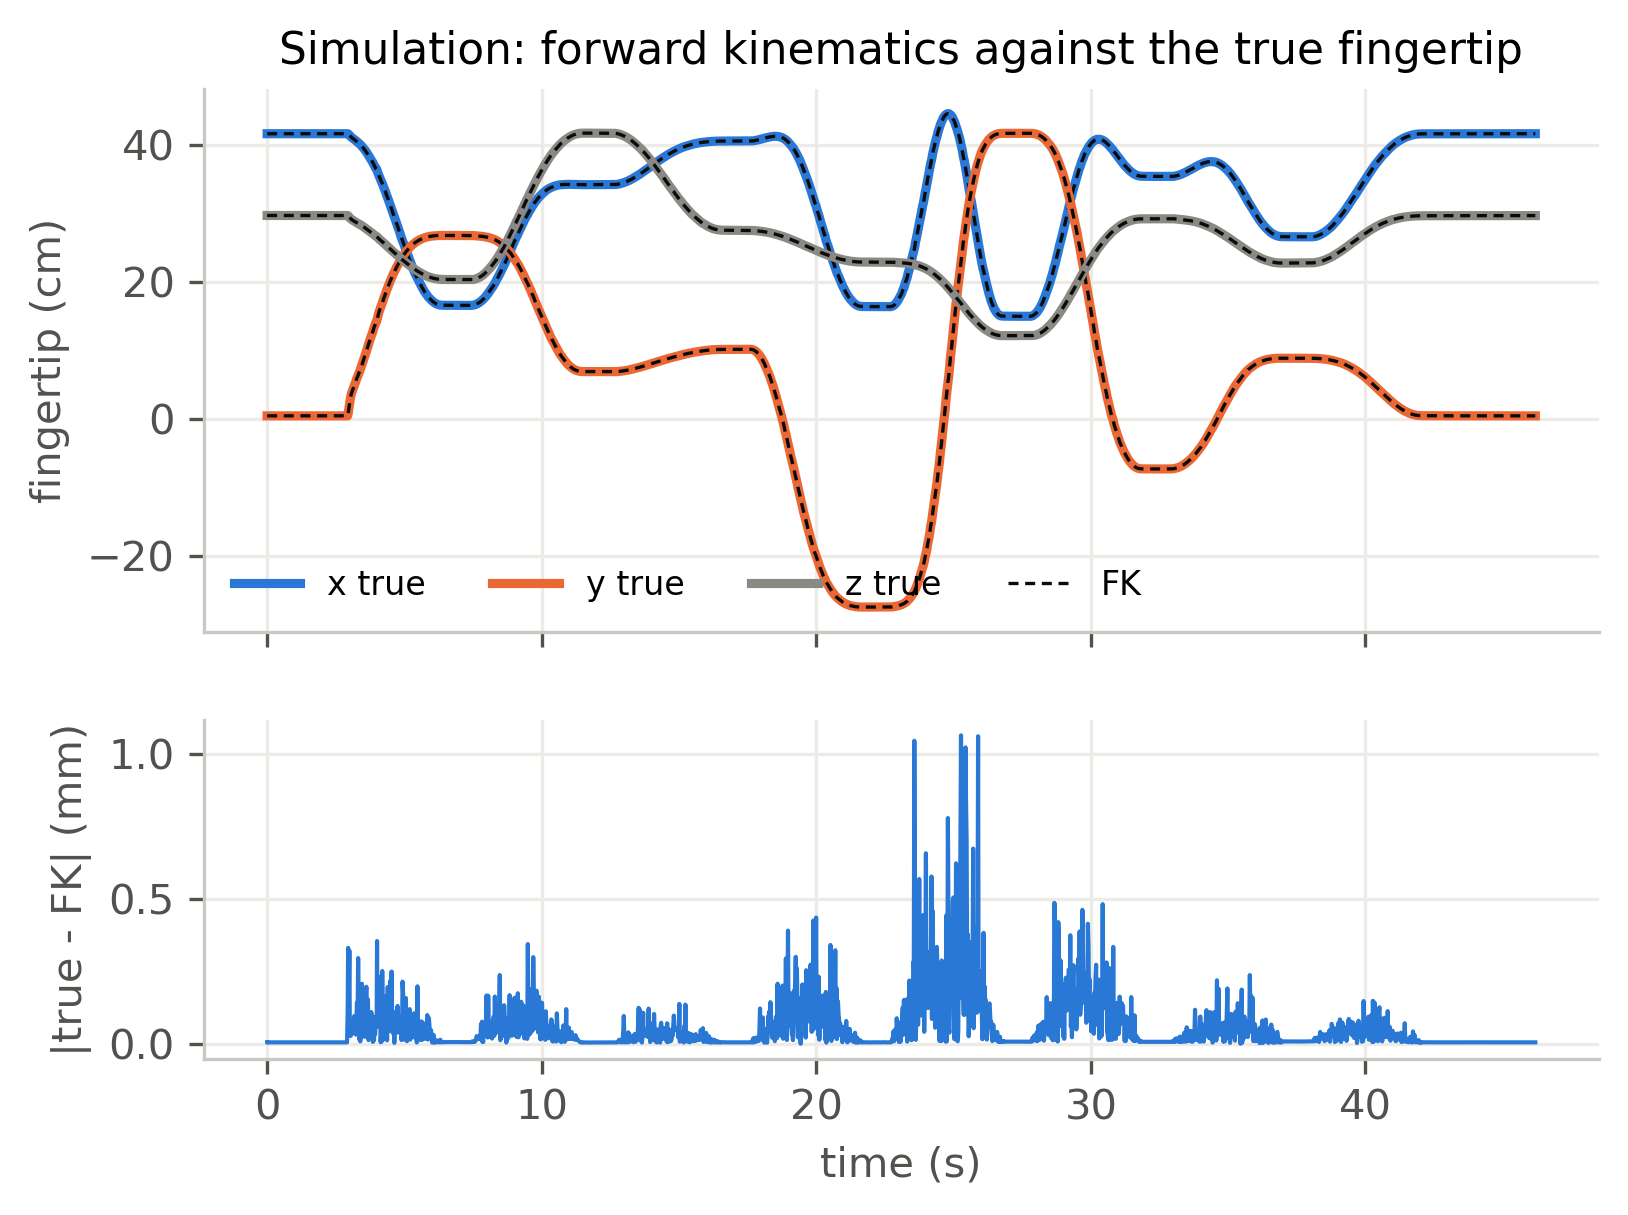
\includegraphics[width=\columnwidth]{figures/fk_validation.png}
\caption{FK validation in simulation. Top: true fingertip coordinates (solid) and FK estimate (dashed). Bottom: model error $e_{mod}$~\eqref{eq:emod}.}
\label{fig:fk}
\end{figure}

\subsection{Typing accuracy in simulation}
All three simulated keys registered. Fig.~\ref{fig:poserr} shows the position error~\eqref{eq:epos} at the deepest point of each press: 5.9~mm for \texttt{a}, 5.5~mm for \texttt{s} and 5.9~mm for \texttt{d}. The error is nearly the same for all three keys and consists of a $-4.7$~mm offset in $x$ (the finger stops short of the target), $-2.8$ to $-3.3$~mm in $z$ and at most 1.5~mm in $y$, so it is a systematic offset.

Fig.~\ref{fig:modtrk} separates this error into its two sources. The model error~\eqref{eq:emod} is 0.01~mm, while the tracking error~\eqref{eq:etrk} is 5.5--5.9~mm. Almost all of the position error is tracking error, meaning the simulated position servos did not reach the angles that IK commanded. The most likely cause is the contact force, as the key spring pushes back on the finger while the position controllers have finite stiffness. The fingertip point also ended about 3~mm below the commanded depth. We attribute this to the finger body contacting the key slightly away from the modelled tip point. The total error stayed below the 8~mm press margin $\delta_p$, so every key still registered.

\begin{figure}[t]
\centering
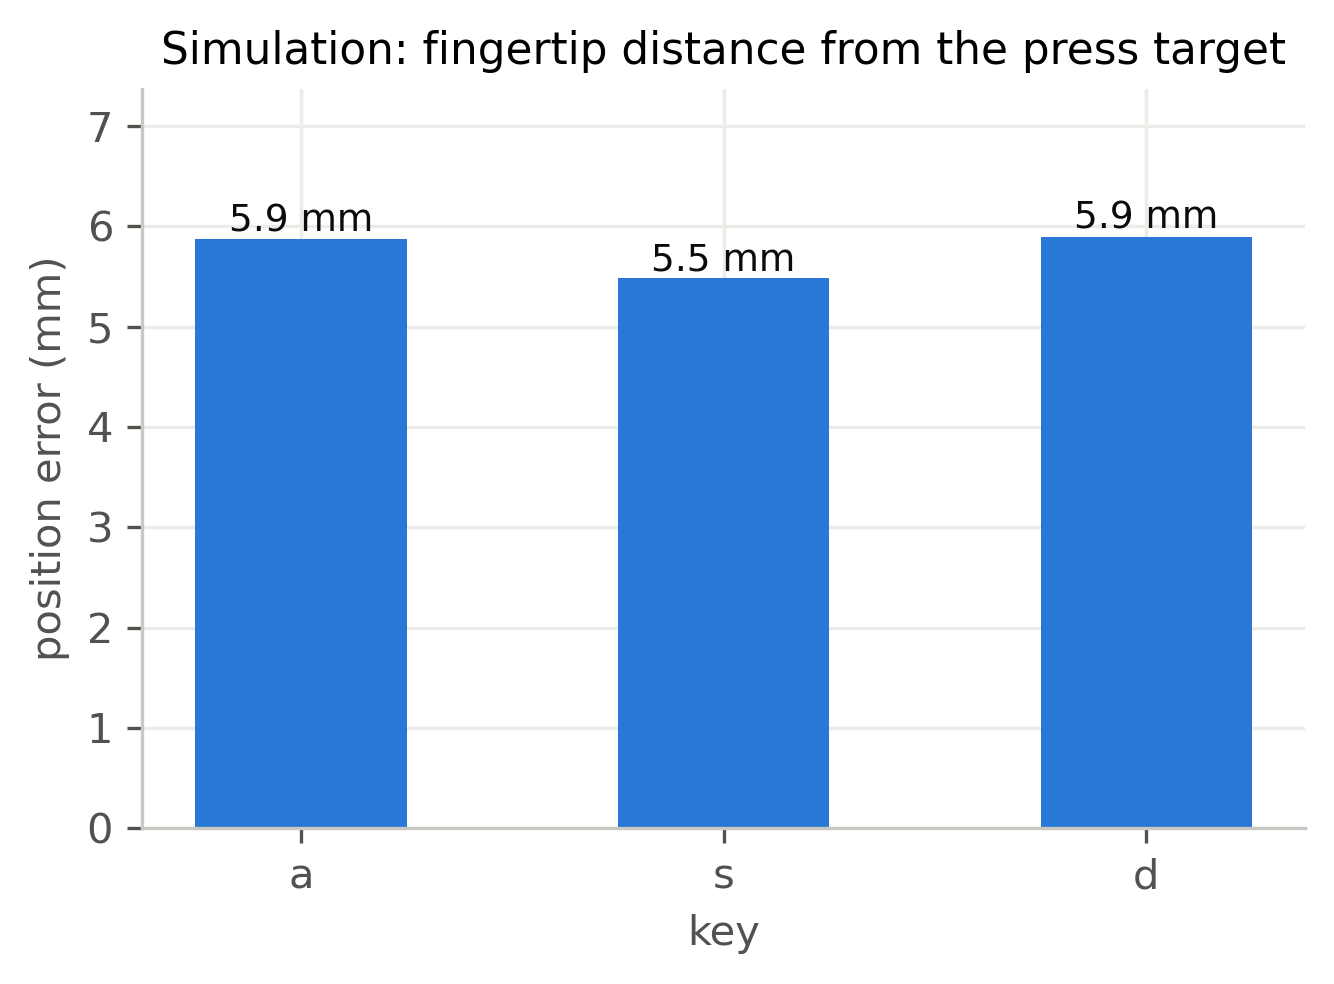
\includegraphics[width=0.92\columnwidth]{figures/position_error.png}
\caption{Simulation: position error $e_{pos}$~\eqref{eq:epos} between the true fingertip and the press target, for each key.}
\label{fig:poserr}
\end{figure}

\begin{figure}[t]
\centering
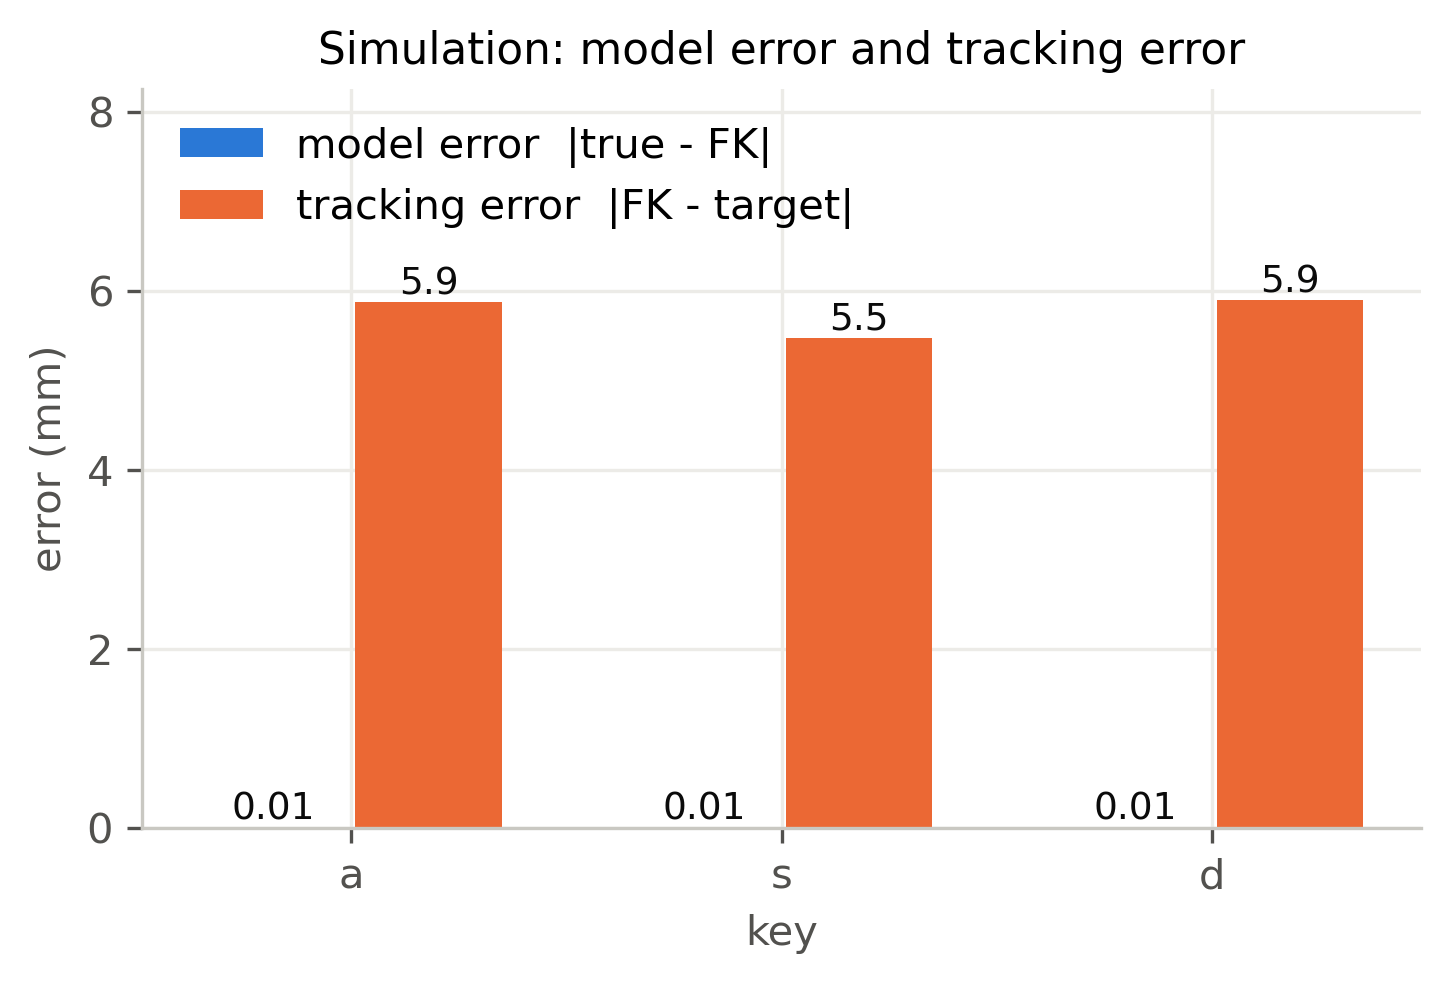
\includegraphics[width=0.95\columnwidth]{figures/model_vs_tracking.png}
\caption{Simulation: model error $e_{mod}$~\eqref{eq:emod} versus tracking error $e_{trk}$~\eqref{eq:etrk} for each key.}
\label{fig:modtrk}
\end{figure}

\subsection{Speed versus success}
Fig.~\ref{fig:speed} shows how many of the three keys registered as the move time $T$ was reduced. For $T\geq0.25$~s, all three keys registered. At $T=0.15$~s only one did, and at $T=0.1$~s none did. At these speeds the commanded trajectory~\eqref{eq:interp} outruns the servos. The press waypoint is replaced by the next hover command before the finger has pushed the key the required 3~mm. The speed limit therefore comes from the actuators, and lies between 0.25 and 0.15~s per move (0.75 to 0.45~s per key).

\begin{figure}[t]
\centering
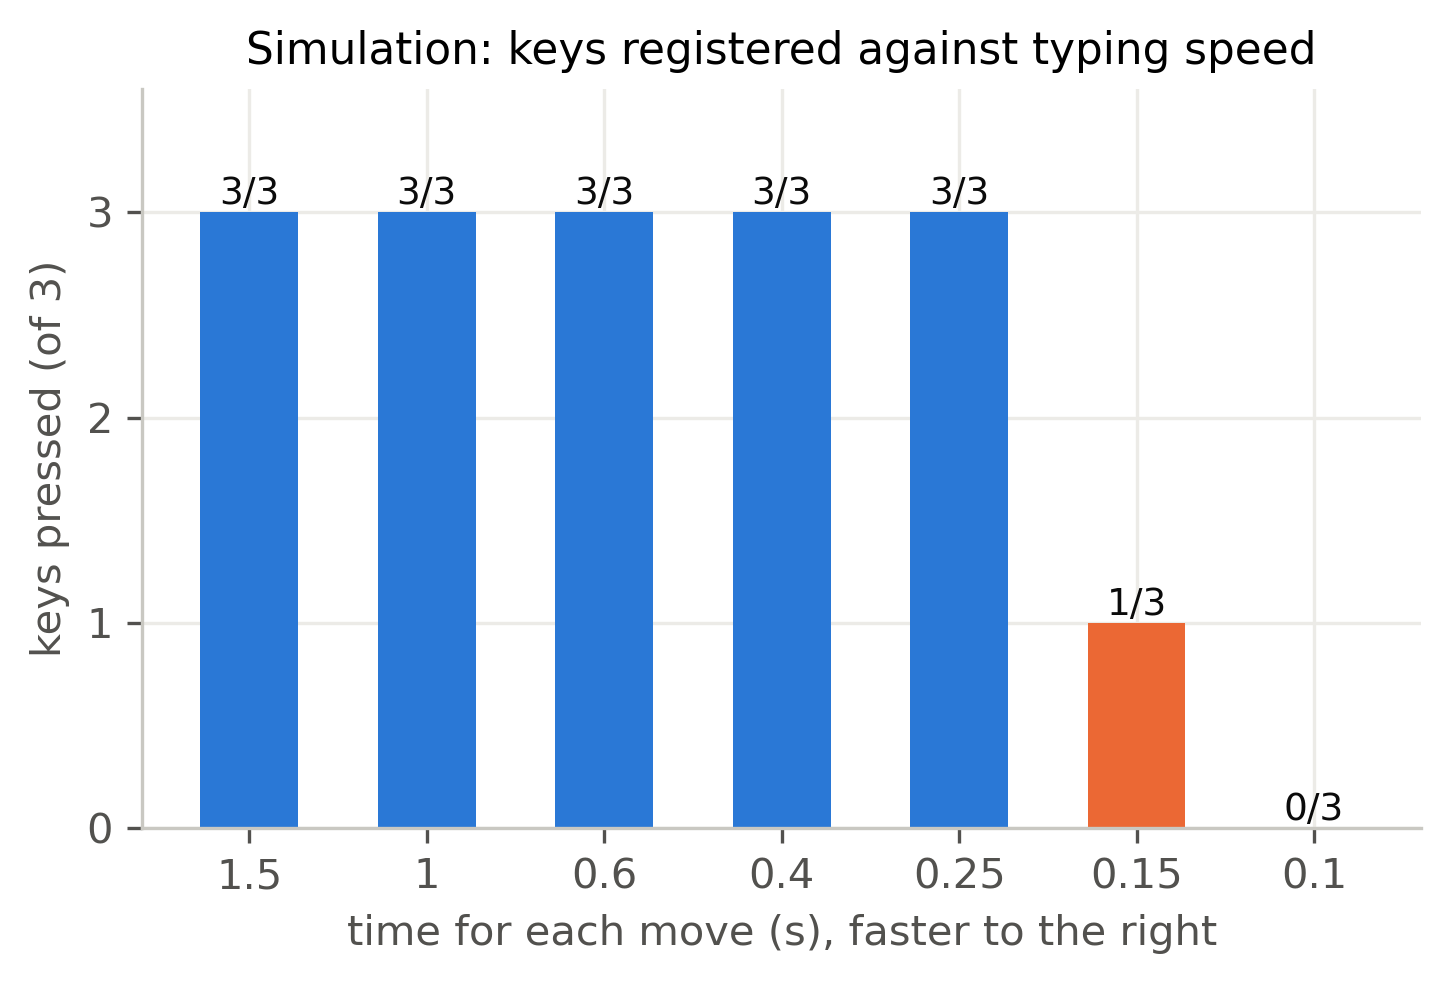
\includegraphics[width=0.95\columnwidth]{figures/speed_vs_success.png}
\caption{Simulation: number of keys registered (of 3) against the move time $T$ of~\eqref{eq:interp}. Orange bars mark failures.}
\label{fig:speed}
\end{figure}

\subsection{Typing on the real robot}
The robot typed ``pool'' correctly, with four of four letters. Fig.~\ref{fig:real} shows the fingertip height computed by FK during the run, and Table~\ref{tab:real} gives the settled positions. Every press settled within 2.1--4.1~mm of its target, and within 2~mm in height. This is similar to the simulated accuracy even though the real arm has backlash and a different geometry from the model, which suggests that measuring the keys with the robot's own FK removed most of the model error.

The lifts were much less accurate. Home was commanded at $z=33$~mm, but even at the start the arm only reached 19~mm. After the presses on \texttt{p} and \texttt{o}, it rose only to $-3$~mm, which is 43--44~mm short of home, and it stayed there until the next command. The driver log showed the shoulder-lift servo stuck about $8^\circ$ short of its command, with the step limit~\eqref{eq:clamp} active at every cycle. Lifting raises the arm against gravity with the shoulder servo, and two factors left that servo too weak. First, the step limit caps the commanded lead, and with it the servo effort. Second, the servo supply measured only 10.1~V instead of the nominal 12~V. Descending motions, which gravity assists, reached their targets. The final lift after \texttt{l} reached 18~mm, because from that key the shoulder barely has to move. Typing still succeeded because a lift of 14~mm is enough to release a laptop key. The cycle time was 7.2--10.9~s per letter, dominated by the slow, clamped motions and the script's wait times.

\begin{figure*}[t]
\centering
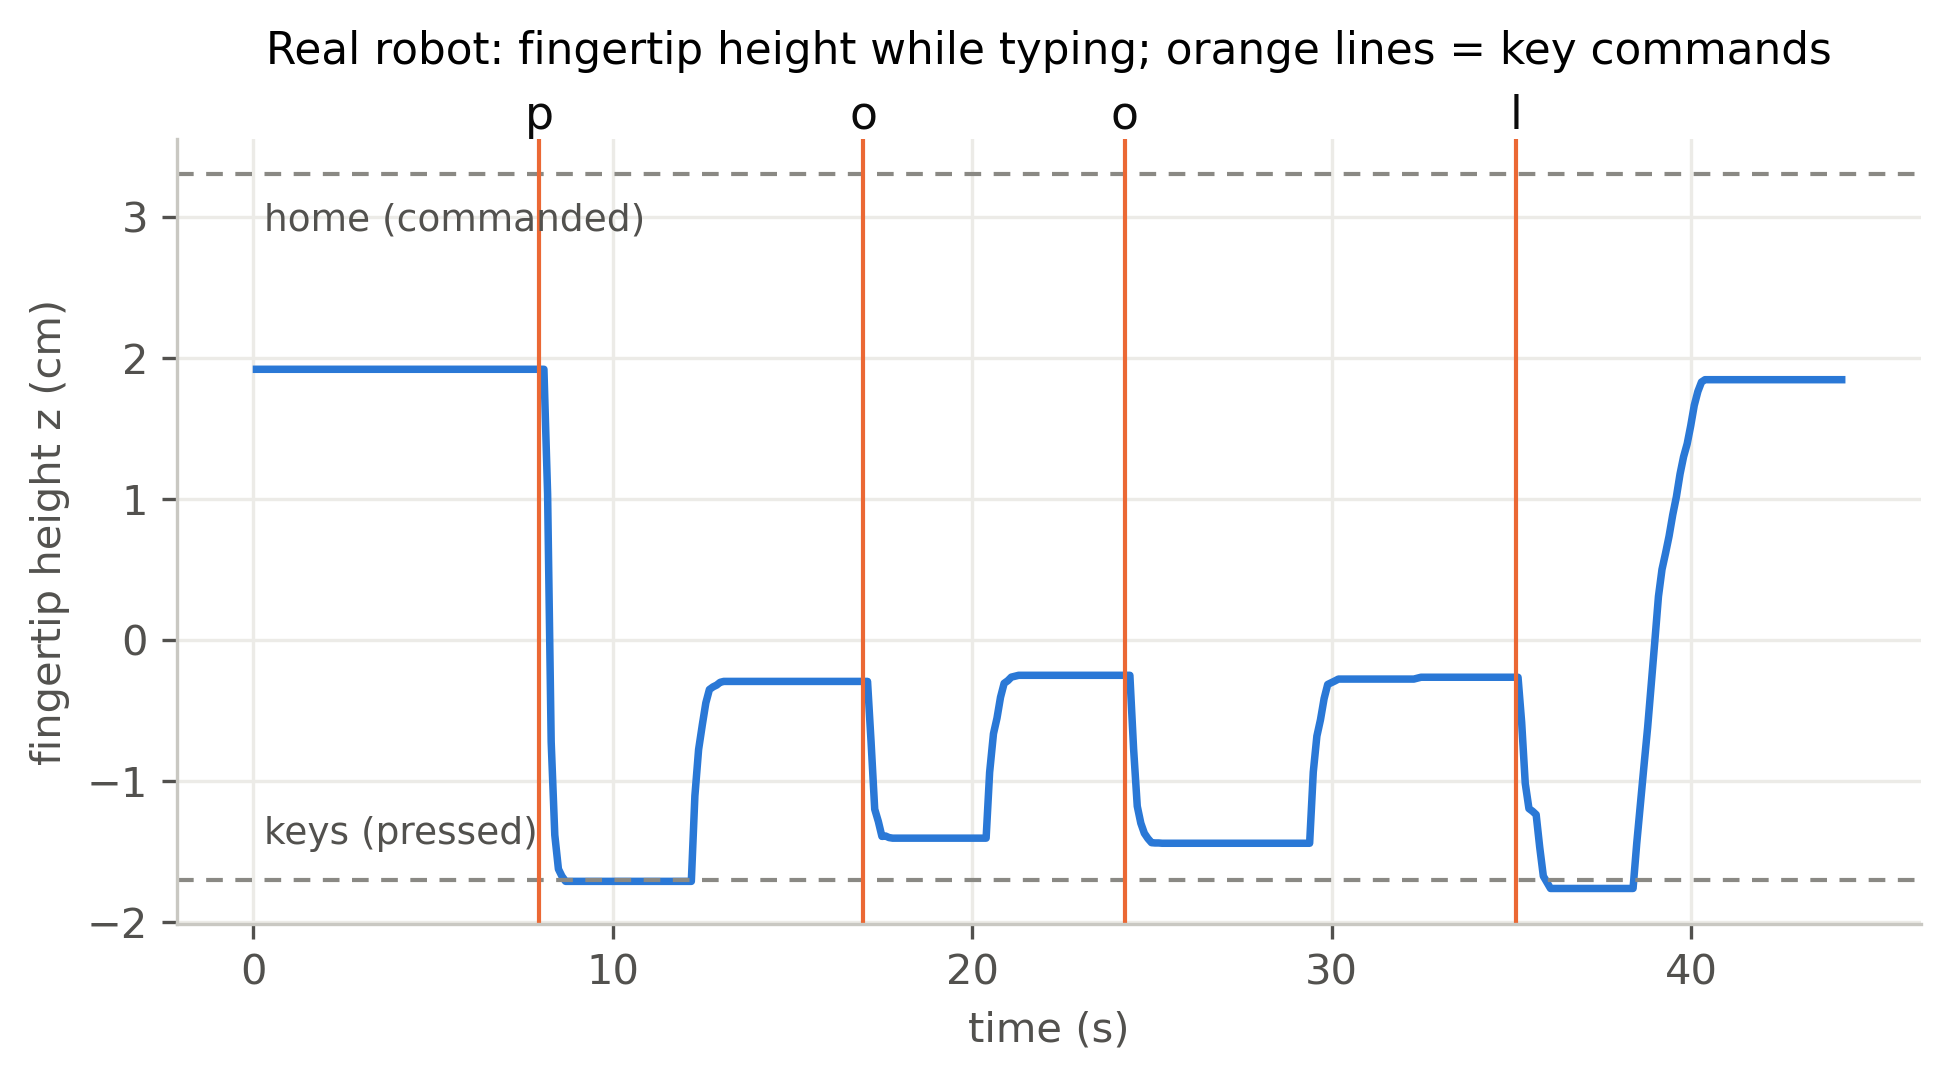
\includegraphics[width=0.8\textwidth]{figures/real_typing_height.png}
\caption{Real robot typing ``pool'': fingertip height from FK. Orange lines mark the key commands, and home is commanded after every key. The lower dashed line is the measured key height, and the upper dashed line is the commanded home height.}
\label{fig:real}
\end{figure*}

\begin{table}[t]
\centering
\caption{Real robot: where the fingertip settled (FK) after each command}
\label{tab:real}
\resizebox{\columnwidth}{!}{%
\begin{tabular}{@{}llll@{}}
\toprule
Cmd. & Target (m) & Settled (m) & Error (mm) \\
\midrule
\texttt{p} & $(0.293, 0.115, -0.018)$ & $(0.289, 0.115, -0.017)$ & 4.1 \\
\texttt{o} & $(0.280, 0.136, -0.016)$ & $(0.281, 0.135, -0.014)$ & 2.8 \\
\texttt{o} & $(0.280, 0.136, -0.016)$ & $(0.281, 0.134, -0.014)$ & 2.5 \\
\texttt{l} & $(0.269, 0.124, -0.017)$ & $(0.269, 0.122, -0.018)$ & 2.1 \\
\midrule
home (start) & $(0.281, 0.125, 0.033)$ & $(0.269, 0.121, 0.019)$ & 18.5 \\
home (after \texttt{p}, \texttt{o}) & $(0.281, 0.125, 0.033)$ & $(0.259, 0.115, -0.003)$ & 43.0--43.6 \\
home (end) & $(0.281, 0.125, 0.033)$ & $(0.270, 0.121, 0.018)$ & 18.6 \\
\bottomrule
\end{tabular}}
\end{table}

\subsection{Assumptions and problems}
The real-robot accuracy figures rest on FK, which agrees with the true fingertip only up to the SO-100/SO-101 mismatch. They measure repeatability relative to the measured keys and say little about absolute accuracy. The key positions are valid for one placement of the robot and keyboard. When the keyboard was moved during testing, the keys had to be measured again. The first key layout, beside the robot at $y\approx0.36$~m, was outside the region reachable with a vertical finger, so the robot was turned to face the keyboard. Earlier, with the arm stretched far, the shoulder and elbow servos tripped their overload protection. Targets were sent as single messages, and a message published before all subscribers had connected was occasionally lost. This was solved by waiting for every subscriber before publishing.

% =====================================================================
\section{Conclusion}
\label{sec:conclusion}
We built a ROS~2 task-space controller for the LeKiwi arm from a rotation-chain FK model and a damped-least-squares IK solver, and we used it to type on a keyboard. The kinematics worked well. FK matched the simulator's ground truth with a median error of 0.02~mm over a 45~s trajectory, and IK found a vertical-finger solution within the 5~mm tolerance for every reachable target. Most of the remaining error came from the actuators. In simulation, 5.5--5.9~mm of positioning error came almost entirely from servo tracking, and typing failed once a move took less than 0.25~s. On the real robot, presses were accurate to 2.1--4.1~mm and all four letters of ``pool'' were typed correctly. Lifts, however, fell up to 44~mm short of their target because the shoulder could not lift against gravity under the driver's 5$^\circ$ step limit and a 10.1~V supply, and each letter took 7--11~s. Restoring the 12~V supply and adding gravity compensation, or closing the loop in task space by correcting the IK target with the FK error, should remove the lift deficit and allow shorter move times.

\bibliographystyle{IEEEtran}
\bibliography{refs}

\end{document}
